\documentclass{article}

\usepackage{amsmath}
\usepackage{amsfonts}
\usepackage{amssymb}
\usepackage{multicol}

\usepackage{mathenv}

\def\nbOne{{\mathchoice {\rm 1\mskip-4mu l} {\rm 1\mskip-4mu l}
{\rm 1\mskip-4.5mu l} {\rm 1\mskip-5mu l}}}

\usepackage{vmargin}
\setmarginsrb{2.5cm}{2.5cm}{2.5cm}{2.5cm}{0cm}{0cm}{0cm}{0cm}

\usepackage[utf8]{inputenc}

\usepackage[french]{babel}
\selectlanguage{french}

\usepackage{color}
\usepackage{graphicx}
\graphicspath{{img/}} 
\usepackage{listings}
\definecolor{colKeys}{rgb}{0.75,0,0}
\definecolor{colIdentifier}{rgb}{0,0,0}
\definecolor{colComments}{rgb}{0.75,0.75,0}
\definecolor{colString}{rgb}{0,0,0.7}

\lstset{
basicstyle=\ttfamily\small, %
identifierstyle=\color{colIdentifier}, %
keywordstyle=\color{colKeys}, %
stringstyle=\color{colString}, %
commentstyle=\color{colComments}, %
showspaces=false,
}
\lstset{language=java}

% Commandes personnelles %

\definecolor{darkred}{rgb}{0.85,0,0}
\definecolor{darkblue}{rgb}{0,0,0.7}
\definecolor{darkgreen}{rgb}{0,0.6,0}
\definecolor{darko}{rgb}{0.93,0.43,0}
\newcommand{\dred}[1]{\textcolor{darkred}{\textbf{#1}}}
\newcommand{\dgre}[1]{\textcolor{darkgreen}{\textbf{#1}}}
\newcommand{\dblu}[1]{\textcolor{darkblue}{\textbf{#1}}}
\newcommand{\dora}[1]{\textcolor{darko}{\textbf{#1}}}
\newcommand{\gre}[1]{\textcolor{darkgreen}{#1}}
\newcommand{\blu}[1]{\textcolor{darkblue}{#1}}
\newcommand{\ora}[1]{\textcolor{darko}{#1}}
\newcommand{\red}[1]{\textcolor{darkred}{#1}}
\newcommand{\ceil}[1]{\left\lceil #1 \right\rceil}
\newcommand{\cdil}[1]{\left\lfloor #1 \right\rfloor}
\newcommand{\image}[1]{\includegraphics{#1}}
\newcommand{\imageR}[2]{\includegraphics[width=#2px]{#1}}
\newcommand{\imageRT}[2]{\includegraphics[height=#2px]{#1}}
\newcommand{\img}[1]{\begin{center}\includegraphics[width=400px]{#1}\end{center}}
\newcommand{\imag}[1]{\begin{center}\includegraphics{#1}\end{center}}
\newcommand{\imgR}[2]{\begin{center}\includegraphics[width=#2px]{#1}\end{center}}
\newcommand{\imgRT}[2]{\begin{center}\includegraphics[height=#2px]{#1}\end{center}}
\newcommand{\point}[2]{\item \ora{\underline{#1}} : \textit{#2}}
\newcommand{\bfp}[2]{\item \textbf{#1} : \textit{#2}}
\newcommand{\sumparam}[3]{\sideset{}{_{#1}^{#2}}\sum{#3}}
\newcommand{\sumin}[3]{\sideset{}{_{i=#1}^{#2}}\sum{#3}}
\newcommand{\sumkn}[3]{\sideset{}{_{k=#1}^{#2}}\sum{#3}}
\newcommand{\intin}[3]{\sideset{}{_{#1}^{#2}}\int{#3}}
\newcommand{\stitre}[1]{\noindent\textbf{\underline{#1}} \\}
\newcommand{\R}{\mathbb{R}}
\newcommand{\Z}{\mathbb{Z}}
\newcommand{\N}{\mathbb{N}}
\DeclareMathAlphabet{\mathpzc}{OT1}{pzc}{m}{it}

\title{\textbf{\textcolor{darkblue}{Structures de Données - Résumé Janvier 2010.}}}
\author{\textit{Dubuc Xavier}}

\begin{document}

\maketitle

\hbox{\raisebox{0.4em}{\vrule depth 0.4pt height 0.4pt width 10cm}}

\tableofcontents

$ $ \\
\hbox{\raisebox{0.4em}{\vrule depth 0.4pt height 0.4pt width 10cm}}

\newpage

\section{Récapitulation des complexités}

\subsection{Recherche}

\begin{tabular}{|*{3}{c|}}
	\hline
	\dred{Structures de données} & \dred{Pire des cas} & \dred{Moyenne} \\
	\hline
	Listes non-triées  & $\approx n$ & $\approx n$ \\
	\hline
	Listes triées  & $\approx n$ & $\approx \frac{n}{2}$\\
	\hline
	ABR & $\approx n$ & $\approx 2\ln{(n)}$ \\
	\hline
	Arbres AVL & \gre{$\approx log_2{(n)}$} & /\\
	\hline
	Tas (recherche de max) & \gre{$\approx 1$} & /\\
	\hline
	Tables de hachage & $\approx n$ & $\approx \frac{l}{2}$ ($l =$ taille de la liste)\\
	\hline
\end{tabular}

\subsection{Tri (recherche avec succès)}

\begin{tabular}{|*{3}{c|}}
	\hline
	\dred{Structures de données} & \dred{Pire des cas} & \dred{Moyenne} \\
	\hline
	Listes non-triées  & $\approx n^2$ & $\approx \frac{n^2}{2}$ \\
	\hline
	Listes triées  & $\approx n^2$ & $\approx \frac{n^2}{2}$\\
	\hline
	ABR & $\approx n^2$ & $\approx n(2\ln{(n)})$\\
	\hline
	Arbres AVL & \gre{$\approx nlog_2{(n)}$} & /\\
	\hline
	Tas & \gre{$\approx nlog_2{(n)}$} & /\\
	\hline
\end{tabular}

\subsection{Tri (recherche avec échec)}

\begin{tabular}{|*{3}{c|}}
	\hline
	\dred{Structures de données} & \dred{Pire des cas} & \dred{Moyenne} \\
	\hline
	Listes non-triées  & $\approx n^2$ & $\approx n^2$ \\
	\hline
	Listes triées  & $\approx n^2$ & $\approx \frac{n^2}{2}$\\
	\hline
	ABR & $\approx n^2$ & $\approx n(2\ln{(n)}+2)$ \\
	\hline
	Arbres AVL & \gre{$\approx nlog_2{(n)}$} & /\\
	\hline
	Tas & \gre{$\approx nlog_2{(n)}$} & /\\
	\hline
\end{tabular}

\section{Notions \& Idées}

\subsection{Chapitre 2 - Arbres Binaires}

\noindent\underline{Définition récursive} : Hauteur d'un noeud :
\begin{itemize}
\item Hauteur des feuilles : 1
\item Si un noeud a 2 fils d'hauteur respective $h$ et $h'$, alors ce noeud a une hauteur de $max(h,h')+1$ \\
\end{itemize}

\noindent\underline{Définition récursive} : Profondeur d'un noeud :
\begin{itemize}
\item Profondeur de la racine : 0
\item Si un noeud a une profondeur $p$, alors ses fils ont une profondeur de $p+1$. \\
\end{itemize}

\noindent\textbf{\underline{Propriété}} : pour un arbre binaire à $n$ noeuds de hauteur $h$, on a : \red{$h\leq 
n\leq2^{h}-1$} et \red{$log_2(n+1)\leq h\leq n$}.
\underline{Preuve} : Fixons $h$,\\
\begin{itemize}
\item recherchons le nombre minimum $n_{min}$ de noeuds d'un arbre binaire de hauteur $h$ : 
\begin{lstlisting}
o                  o                    o
 \                  \                  /
  o                  o                o
  ...         ou    /       ou      ...
    \              ...              /
     o               \             o
                      o
\end{lstlisting}
C'est-à-dire pour tout noeud qui n'est pas une feuille, ce noeud possède un seul fils ; \\on a donc $n_{min}=h$.
\item recherchons le nombre maximum $n_{max}$ de noeuds d'un arbre binaire de hauteur $h$ : 
\begin{lstlisting}
       o               niveau 1 : 1 noeud  (= 2^(1-1))
     /   \
    o     o            niveau 2 : 2 noeuds (= 2^(2-1))
   / \   / \
      ...
 / \       / \ 
o   o ... o   o        niveau n : 2^(h-1) noeuds
\end{lstlisting}

On a donc $n_max = 2^0+2^1+...2^{h-1} = \dfrac{2^k-2^0}{2-1} = 2^h-1$
\end{itemize}

\noindent De tout ça on tire facilement que pour un arbre de hauteur $h$ et de $n$ noeuds, on a $n_{min} \leq n 
\leq n_{max}$ et donc : \red{\begin{center}$\boxed{h \leq n \leq 2^{h}-1}$\end{center}}
De plus, comme on a $n\leq 2^h-1$ et ceci étant équivalent à $n+1 \leq 2^h$ on peut écrire :  
\red{\begin{center}$\boxed{\log_2{(n+1)} \leq h}$\end{center}}

\noindent\textbf{\underline{Propriété}} : Soit un arbre binaire à $n$ noeuds de hauteur $h$, soit $n_I$ le 
nombre de noeuds internes qu'il possède et $n_F$ le nombre de feuilles (donc $n_I+n_F=n$) on a \red{$1\leq 
n_F\leq 2^{h-1}$} et \red{$h-1 \leq n_I \leq 2^{h-1} -1$}.\\
\underline{Preuve} : on procède comme pour la preuve précédente, \\

\begin{lstlisting}
o                            o
 \                         /   \
  o                       o     o
  ...                    / \   / \
    \    nI = h-1          ...        nF = 2^(h-1) 
     o   nF = 1       / \       / \   nI = 2^h - 1 - 2^(h-1) = 2^(h-1) - 1
                     o   o ... o   o
\end{lstlisting}

\noindent\textit{\underline{Remarque}} : $n_I$ correspond au nombre de noeud d'un arbre de hauteur $h-1$. \\

\noindent\underline{Définition} : $T$, arbre binaire, $C(T)$ son complété, on définit :
\begin{itemize}
\item \textit{Internal path length}(\textbf{IPL}) : $I(T)$ : somme des profondeurs des noeuds internes de T.
\item \textit{External path length}(\textbf{EPL}) : $E(T)$ : somme des profondeurs des feuilles de T.
\end{itemize}

\noindent On a $E(T) = I(T)+2n$, \\

\noindent\underline{Preuve} : \\
Calculons de 2 façons $\sideset{}{_{v\ noeuds\ de\ C(T)}}\sum{prof(v)}$ : \\
(1) $ = \sideset{}{_{v\ noeuds\ internes\ de\ C(T)}}\sum{prof(v)} + \sideset{}{_{v\ feuilles\ de\ 
C(T)}}\sum{prof(v)} $ \\
\indent    $\ = \sideset{}{_{v\ noeuds\ de\ T}}\sum{prof(v)} + \sideset{}{_{v\ feuilles\ de\ C(T)}}\sum{prof(v)} 
= I(T)+E(T)$ \\
(2) $ = prof(racine) + \sideset{}{_{v\ noeuds\ de\ T}}\sum{2\left(prof(v)+1\right)} = 0 + 2
\sideset{}{_{v\ noeuds\ de\ T}}\sum{prof(v)} + 2n$

\noindent\underline{\textit{Explications}} : tout noeud de $C(T)$ est le fils d'un noeud interne de $C(T)$ c'est-
à-dire un noeud de $T$ (sauf la racine), de plus, tout noeud interne de $C(T)$ a 2 fils par définition.

\noindent $(1)=(2)\Rightarrow I(T)+E(T) = 2n+2I(T) \Rightarrow \boxed{\textcolor{darkred}{E(T) = I(T) + 2n}}$ \\

Prouvons que $(n+1) \log_2\left\{\dfrac{(n+1)}{4}\right\} < I(T) \leq \dfrac{n(n-1)}{2}$, \\

On s'interesse à un arbre qui a un nombre minimum de noeuds, et à un arbre qui a un nombre maximum de noeuds.

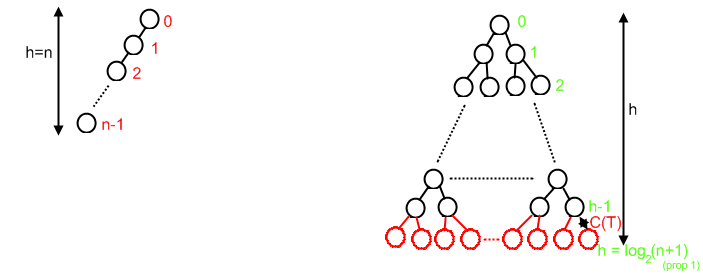
\includegraphics[width=300px]{img2.png}

\noindent\underline{Premier dessin} : \\ $I(T) = 0+1+...+(n-1) = \dfrac{(n-1)n}{2}$ \\
\underline{Second dessin} : \\ $I(T) = E(T) - 2n$ \\
$ = \sideset{}{_{v\ noeuds\ de\ C(T)}}\sum{prof(v)} = \sideset{}{_{v\ feuilless\ de\ C(T)}}\sum{\log_2(n+1)}$ \\
$ = (n+1)\log_2(n+1)-2n$ \\

\noindent\underline{En général : } \\
$(n+1)\log_2(n+1)-2n \leq I(T) \leq \dfrac{(n-1)n}{2} \\
(n+1)\log_2(n+1)-2(n+1) < I(T)  \\ 
(n+1) \left[ \log_2(n+1) - 2 \right] < I(T) \\
(n+1) \left[ \log_2(n+1) - \log_2(4) \right] < I(T)  \\
(n+1) \log_2\left(\dfrac{(n+1)}{4} \right) < I(T) \\$

\dred{$\rightarrow h$ a une complexité comprise entre $\log_2n$ et $n$ et I(T) entre $n\ \log_2n$ et $n^2$.} \\

Soit $T$ un arbre binaire ayant $n$ noeuds alors son complété $(C(T))$ a $2n+1$ noeuds. \textit{En particulier, 
$T$ a $n+1$ références vides)}

\noindent\underline{Preuve} :

$C(T)$ a des feuilles qui correspondent aux références vides de $T$, il a $n$ noeuds internes, 2 fils par noeuds 
pour tout noeud qui ne sont pas des feuilles ; il a donc au total $n+m$ noeuds. A part la racine, tout noeud est 
fils d'un certains noeud interne donc $C(T)$ a $1$(racine)$+2n$ (les $2$ fils de chacun des $n$ noeuds internes).
\textbf{On a donc $m+n = 2n+1$ et donc $\boxed{m=n+1}$.} \\
Quant aux arbres $k$-aires, $\boxed{\dred{C(T)\ a\ kn+1}}$ noeuds et $\boxed{\dred{T\ a\ (k-1)n+1}}$ références 
vides.

\subsection{Chapitre 3 - ABR}

\noindent L'\textbf{IPL} d'un \textbf{ABR} vaut en moyenne $2n\ln{(n)}$ et comme $\mathbf{EPL} = 
\mathbf{IPL}+2n$, on a que $\mathbf{EPL} = 2n\ln{(n)}+2n$.

\noindent\underline{Preuve} : rappellons nous que dans le $ (n+1) \log_2{(\frac{n+1}{4})}\leq I_n \leq 
\frac{n(n-1)}{2}$ \\
On va calculer $I_n$ moyen par récurrence : \\
$I_1 = 0\\
I_2 = ...
I_3 = \frac{8}{3}$ (cf. exemple du cours) \\
...
$I_n = ?$ \\
\begin{enumerate}
\item Fixons une donnée $k$ telle que $1 \leq k \leq n$ et supposons qu'elle soit racine, on a donc le schéma :
\begin{lstlisting}
T ->  k
     / \   (remarque : si prof(f) = x dans T1 ou T2 alors prof(f) = x+1 dans T)
    T1 T2
\end{lstlisting}
\textit{$T_1$ contient les données allant de $1$ à $k-1$ et $T_2$ de $k+1$ à $n$.} \\
On exprime $I(T)$ en fonction de $I(T_1)$ et $I(T_2)$ : \\
$ = I(T_1)+(k-1)$\textit{(nombre de noeuds dans $T_1$)}$+I(T_2)+(n-k)$\textit{(nombre de noeuds dans 
$T_2$)}$+prof(racine) \\ = I(T_1)+I(T_2)+(n-1)$

\item Fixons $h$, mais passons à la moyenne pour les 2 sous arbres de $k$ : \\
$I(T) = I_{k-1} + I_{n-k} + (n-1)$ \textit{(= IPL moyen pour un arbre de $k-1$ données)}

\item Passons à une racine quelconque : \\
$\rightarrow$ moyenne : $\frac{1}{n} \sumkn{1}{n}{I_{k-1}+I_{n-k}+(n-1)}$

\end{enumerate}

\noindent\textbf{On cherche à se ramener à une récurrence faible ($I_n = f(I_{n-1})$) :} \\
$I_n = \frac{1}{n}\left(\sumkn{1}{n}{I_{k-1}} + \sumkn{1}{n}{I_{n-k}} + \sumkn{1}{n}{n-1}\right) 
= \frac{2}{n}\left(\sumkn{1}{n}{I_{k-1}}\right) + (n-1) \\$

\noindent\textbf{On calcule $nI_n-(n-1)I_{n-1}$ :} \\
$= \left(2\sumkn{1}{n}{I_{k-1}} + n(n-1)\right) - \left(2\sumkn{1}{n-1}{I_{k-1}} + (n-1)(n-2)\right) \\
= 2 I_{n-1} + n(n-1)-(n-1)(n-2)$ (soustraction des termes identiques dans les 2 sommes) \\
$ = 2 I_{n-1} + (n-1) (n-(n-2)) \\
= 2 I_{n-1} + 2(n-1)) \\$

\noindent On a donc : $nI_n-(n-1)I_{n-1} = 2 I_{n-1} + 2(n-1)) \Rightarrow \boxed{nI_n = (n+1) I_{n-1} + 
2(n-1)}\\$
Divisons par $n(n+1)$ : $\frac{nI_n}{n(n+1)} = \frac{(n+1)I_{n-1}}{n(n+1)} + \frac{2(n-1)}{n(n+1)}$ \\
$\Leftrightarrow \frac{I_n}{n+1} = \red{(}\frac{I_{n-1}}{n}\red{)} + \frac{2(n-1)}{n(n+1)} \\
= \red{(}\gre{(}\frac{I_{n-2}}{n-1}\gre{)} + \frac{2(n-2)}{(n-1)n}\red{)} + \frac{2(n-1)}{n(n+1)}$ (récurrence)\\
$= \red{(}\gre{(}\ora{(}\frac{I_{n-3}}{n-2}\ora{)} + \frac{2(n-3)}{(n-2)n}\gre{)} + \frac{2(n-2)}{(n-1)n}\red{)} 
+ \frac{2(n-1)}{n(n+1)}$ (récurrence) \\
... \\
$ = I_1 + (...) \\
= I_1 + \sumkn{2}{n}{\frac{2(k-1)}{k(k+1)}}$ $(I_1 = 0)$\\

\noindent Au final : $\frac{I_n}{n+1} = \sumkn{2}{n}{\frac{2(k-1)}{k(k+1)}}$\\
On va à présent simplifier les calculs, $\frac{I_n}{n+1} = \sumkn{2}{n}{\frac{2(k-1)}{k(k+1)}} \sim 2 \sumkn{2}
{n}{\frac{k}{kk}} = 2 \sumkn{2}{n}{\frac{1}{k}}$.
On va approcher cette somme par une intégrale semblable : \\
$2 \sumkn{2}{n}{\frac{1}{k}} \sim 2 \intin{1}{n}{\frac{1}{x} dx} = 2 \left[\ln x\right]_1^n = 2(\ln n -\ln 1) = 
2\ln n$ \\

\noindent \textbf{On a donc $\boxed{\frac{I_n}{n+1} \sim \frac{I_n}{n} \sim \red{I_n \sim 2 \ln n}}$}

Vu que $E(T) = I(T) + 2n$, on a $E_n = I_n + 2n \Rightarrow \red{\boxed{E_n = 2n \ln n + 2n}}$. \\

\noindent\textbf{Propriété} : La recherche avec succès dans un \textbf{ABR} demande en moyenne un nombre de 
comparaisons $\sim 2\ln n$. \\
\underline{Preuve} : 
\begin{enumerate}
\item Fixons $k$ une donnée de cet arbre que l'on recherche : \\
\begin{lstlisting}
      o
     /
    o
     \
      o
     /
    k    -> profondeur de k
\end{lstlisting}

Le nombre de comparaisons pour trouver $k$ vaut $prof(k)+1$.
\item en moyenne $\frac{1}{n} \sumkn{1}{n}{prof(k)+1}$ \\
$ = \frac{1}{n} \sumparam{v\ noeuds}{}{prof(v)+1} \\
= \frac{1}{n} \sumparam{v\ noeuds}{}{prof(v)} + \frac{1}{n}\sumparam{v\ noeuds}{}{1} \\
= \frac{I_n}{n} + 1 \\
\sim \frac{2n \ln n}{n} + 1 \\
\sim \red{\boxed{2 \ln{n}}}$
\end{enumerate}

\noindent\textbf{Propriété} : La recherche avec échec dans un \textbf{ABR} demande en moyenne un nombre de 
comparaisons $\sim 2\ln n$. \\

\begin{enumerate}
\item Fixons une référence vide sur laquelle on tombe par une recherche : 
\begin{lstlisting}
      o
     /
    o
     \
      o
     /
    X    -> profondeur ref vide
\end{lstlisting}
\noindent \textit{Le nombre de comparaisons est égal à la profondeur de la référence vide.}
\item En moyenne, sachant qu'on a $n+1$ références vides, \\
$\frac{1}{n+1} \sumparam{r\ ref\ vide}{}{prof(r)} \\
= \frac{1}{n+1} \sumparam{f\ feuilles\ C(T)}{}{prof(feuille)} \\
= \frac{1}{n+1} E_n \\
\sim \frac{2n\ln{(n)}+2n}{n+1} \\
\sim \red{\boxed{2 \ln{n}}}$

\end{enumerate}

\subsection{Chapitre 4 - Arbres AVL}

Un arbre \textbf{AVL} est un arbre binaire de recherche tel que $\forall$ noeud qu'il contient, la balance de ce
noeud est égale à $-1$, $0$ ou $1$. \textit{(La balance étant la différence entre les hauteurs de ses 2 sous-
arbres)} \\

\subsubsection{Les rotations}

\stitre{Rotation gauche}

\begin{lstlisting}
  k                  l
 / \        rg      / \
R   l      ====>   k   U
   / \            / \
  S   U          R   S
\end{lstlisting}

\stitre{Rotation droite}

\begin{lstlisting}
    k                l
   / \      rd      / \
  l   R    ====>   U   k
 / \                  / \
U   S                S   R
\end{lstlisting}

\stitre{Rotation double gauche}

\begin{lstlisting}
  k                   m
 / \       drg      /   \
R   l      ====>   k     l
   / \            / \   / \
  m   V          R  S  U   V
 / \            
S   U           
\end{lstlisting}

\noindent\textit{On met le noeud le plus bas comme nouvelle racine, l'ancienne racine comme son fils gauche et le 
noeud «du milieu» comme fils droit ; ensuite on recopie dans l'ordre les sous arbres que l'on place comme les
fils des 2 fils de la racine. Résulte d'une rotation droite sur le sous arbre droit de $k$ suivi d'une rotation 
gauche sur l'arbre entier.}

\newpage

\stitre{Rotation double droite}

\begin{lstlisting}
    k                 m
   / \     drg      /   \
  l   R    ====>   k     l
 / \              / \   / \
V   m            V  S  U   R
   / \            
  S   U 
\end{lstlisting}

Le \textbf{théorème de rééquilibrage} nous dit : \\
Soit $T$ un arbre binaire de recherche non-vide tel que $T$ est formé d'une racine avec 2 fils $T_1$ et $T_2$ 
tous deux des arbres \textbf{AVL} et $bal(T) \in \{-2,-1,0,1,2\}$, on définit $p(T)$ comme :
\begin{itemize}
\item si $bal(T) = 2$ et $bal(T_2) \geq 0\ \ \Rightarrow p(T) = rg(T)$,
\item si $bal(T) = 2$ et $bal(T_2) =-1\Rightarrow p(T) = drg(T)$,
\item si $bal(T) = -2$ et $bal(T_1) \leq 0\Rightarrow p(T) = rd(T)$,
\item si $bal(T) = -2$ et $bal(T_1) =1\Rightarrow p(T) = drd(T)$,
\item si $bal(T) \in \{-1,0,1\}\ \ \ \ \ \ \ \ \ \ \ \Rightarrow p(T) = T$.
\end{itemize}
alors, $p(T)$ est un arbre \textbf{AVL}.\\
\underline{Preuve} : 
\begin{enumerate}
\item \underline{$bal(T) = 2$ et $bal(T_2) \geq 0$} \\
Il faut montrer que $p(T) = rg(T)$ est un arbre \textbf{AVL} :
\begin{lstlisting}
Avant

           k
     /            \
    /\             l    bal >= 0 (0 ou 1) (le cas represente est le cas ou bal = 0)
   /  \         /     \
  / R  \       /\     |\
 /      \     /  \    | \
/------- \   /    \   |  \
            /   S  \  | U \
           /--------\ |----\
           
Apres           

                l (bal = -1) (mais peut aussi etre = 0 selon les cas)
           /          \
          k (bal = 1) |\ (mais peut aussi etre = 0 selon les cas)
     /         \      | \
    /\         /\     |  \                
   /  \       /  \    |   \              
  / R  \     /    \   |    \
 /      \   /   S  \  | U   \
/------- \ /        \ |------\  
          /----------\ 
           
\end{lstlisting}

\textit{(Les arbres ne sont pas grossis réellement, ils le sont juste pour les besoins du dessin, afin 
d'illustrer les tailles différentes, on voit ainsi que $S$ descend 1 niveau plus bas que $U$ et $R$ après la 
rotation et que $S$ et $U$ étaient 2 niveaux plus bas que $R$ avant la rotation.)} \\

\noindent Pour prouver que $p(T)$ est un arbre \textbf{AVL}, il faut montrer 2 choses :
\begin{enumerate}
\item \underline{$p(T)$ est un arbre binaire de recherche ?} \\
$R$,$S$ et $U$ étaient des arbres binaires de recherche avant la rotation (par hypothèse) et, n'ayant pas été 
modifiés, ils le restent. Ensuite, pour les noeuds $k$ et $l$, on vérifie l'ordre : 
\begin{itemize}
\item avant la rotation : $R<k<S<l<U$
\item après la rotation : $R<K<S<l<U$
\end{itemize}
l'ordre est donc conservé. $p(T)$ est un arbre binaire de recherche.
\newpage
\item \underline{$bal(p(T)) \in \{-1,0,1\}$ ?}\\
$R$,$S$ et $U$ sont des arbres \textbf{AVL} par hypothèses et ne sont pas modifiés donc ils le restent, quant aux 
balances elles sont calculées sur le dessin ci-haut. \textbf{$p(T)$ est donc un arbre AVL}
\end{enumerate}

\item \underline{$bal(T)=2$ et $bal(T_2)=-1$} : il faut montrer que $p(T) = drg(T)$ est un arbre \textbf{AVL} :

\begin{lstlisting}
Avant

  k (balance = 2)
 /           \
|\           l (-1)
| \         /     \
|  \       m (0)  |\
| R \    /   \    | \
|----\  |\   |\   |V \
        |S\  |U\  |---\
        |--\ |--\

Apres

        m(0)
    /       \
   k(0)       l(0) (peuvent valoir egalement respectivement -1 et 1)
 /   \      /   \
|\   |\    |\   |\
|R\  |S\   |U\  |V\
|--\ |--\  |--\ |--\     
\end{lstlisting}

\begin{enumerate}
\item \underline{$p(T)$ de recherche ?} \\
$R$,$S$,$U$,$V$ ok, ordre avant $R<k<S<m<U<l<V$ et ordre après $R<k<S<m<U<l<V$ $\Rightarrow p(T)$ est de 
recherche.
\item \underline{$bal(p(T)) \in \{-1,0,1\}$ ?}\\ 
$R$,$S$,$U$,$V$ ok, pour les 3 noeuds, cf dessin $\Rightarrow p(T)$ \textbf{est un arbre AVL}
\end{enumerate}
\item Les cas où $p(T) = rd(T)$ et $p(T) = drd(T)$ sont les cas symétriques.
\item Le cas où $p(T) = T$ est trivial car il n'y a pas de rotation appliquée. \\
\end{enumerate}

\noindent\textbf{Propriété} : La hauteur des arbres \textbf{AVL} est en $O(log_2n)$.

\noindent\underline{Preuve} : fixons $h$ une hauteur et étudions la forme et le nombre de noeuds des arbres 
\textbf{AVL} de hauteur $h$, avec un nombre minimum de noeuds (noté $n_{min}(h)$)\\
\textit{Exemples} : \\
$h = 0 \rightarrow$ \textbf{AVL} vide $\rightarrow n_{min}(0) = 0$ \\
$h = 1 \rightarrow$ k $\rightarrow n_{min}(1) = 1$ \\
$h = 2$
\begin{lstlisting}
  o     o        o
 /   OU  \  OU  / \
o         o    o   o
\end{lstlisting}
$\rightarrow n_{min}(2) = 2$\\
$h = 3$
\begin{lstlisting}
    o          o          o         o
   / \        / \        / \       / \
  o   o   OU o   o   OU o   o  OU o   o
 /            \            /           \
o              o          o             o 
\end{lstlisting}
$\rightarrow n_{min}(3) = 4$\\
...\\
$h-2 \rightarrow n_{min}(h-2)$ \\
$h-1 \rightarrow n_{min}(h-1)$ \\
$h \rightarrow n_{min}(h) = ?$ \\

\newpage

\begin{lstlisting}
  racine(-1) (-1 ou 1 pour avoir moins de noeuds possibles)
 /         \
|\         |\
| \        | \
|T1\       |T2\
|   \      |---\
|----\
\end{lstlisting}
\textit{$T_1$ et $T_2$ doivent être \textbf{AVL} avec un nombre minimum de noeuds $\rightarrow n_{min}(h) = 
1+n_{min}(h-1)+n_{min}(h-2)$}

\noindent Comparaison avec les nombres de \textbf{Fibonnaci} : 
\begin{center}
	\begin{tabular}{|*{11}{c|}}
	\hline
	h & 0 & 1 & 2 & 3 & 4 & 5 & 6 & 7 & 8 & 9 \\
	\hline
	$n_{min}(h)$ & 0 & 1 & 2 & 4 & 7 & 12 & 20 & 33 & 54 & 88 \\
	\hline
	$f_h$ & 0 & 1 & 1 & 2 & 3 & 5 & 8 & 13 & 21 & 34\\
	\hline
	\end{tabular}
\end{center}
\textit{Il semble que $n_{min}(h) = f_{h+2} - 1$} (récurrence forte), on utilise alors la forme de récurrence 
faible des nombre de \textbf{Fibonnaci} pour caractériser notre nombre $n_{min}$ : $f_h = \frac{1}
{\sqrt{5}}\left(\phi^h-\bar{\phi}^{-h}\right)$ \\ 
On aura donc $n_{min} = \frac{1}{\sqrt{5}}\left(\phi^{h+2}-\bar{\phi}^{-(h+2)}\right) - 1$ (où $\phi = 
\frac{1+\sqrt{5}}{2}$ et $\bar{\phi} = \frac{1-\sqrt{5}}{2}$). \\

On aura donc pour un arbre quelconque de taille $n$, $n \geq n_{min}(h)$ \\
$\Leftrightarrow \frac{1}{\sqrt{5}}\left(\phi^{h+2}-\bar{\phi}^{-(h+2)}\right) - 1 \leq n \\
\Leftrightarrow \phi^{h+2} \leq (n+1) \sqrt{5} + \bar{\phi}^{h+2}\ \ \ \ \ $ ($|\bar{\phi}| \leq 1 
\Leftrightarrow |\bar{\phi}|^{h+2} \leq 1$) \\
$\Leftrightarrow \phi^{h+2} < (n+1) \sqrt{5} + 1 \\ 
\Leftrightarrow \log_2{\left(\phi^{h+2}\right)} < \log_2{\left((n+1) \sqrt{5} + 1\right)} \\
\Leftrightarrow (h+2) \log_2(\phi) < \log_2{\left((n+1) \sqrt{5} + 1\right)} \\
\Leftrightarrow h < \blu{\frac{1}{\log_2(\phi)} \left(\log_2{\left((n+1) \sqrt{5} + 1\right)}\right) - 2}$
(\blu{ce qui est en bleu est en $O(\log_2(n))$}) \\
$\Leftrightarrow \red{\boxed{h = O(\log_2{(n)})}}$
\subsection{Chapitre 5 - Tas}

\noindent\textbf{Propriété} : Hauteur en $O(log_2n)$.\\
\underline{Preuve} : On fixe $h$, la hauteur, on étudie le nombre minimum de noeuds d'un tas de hauteur $h$ :
\begin{lstlisting}
     /\
    /  \
   /    \
  /------\
 o
\end{lstlisting}
\textit{Arbre complet sauf le dernier niveau ne contenant qu'un seul noeud.}\\
On se rappelle qu'un arbre «complet» d'hauteur $h-1$ possède $2^{h-1}-1$ noeuds $\rightarrow$ nombre minimum de 
noeuds $ = (2^{h-1} - 1) + 1$. Pour un nombre quelconque de noeuds $n$ on a : \\
$n \geq (2^{h-1}-1) + 1 = 2^{h-1}$ \\
$\rightarrow 2^{h-1} \leq n \\
\Leftrightarrow log_2{(2^{h-1})} \leq log_2{(n)} \\
\Leftrightarrow h-1 \leq log_2{(n)} \\
\Leftrightarrow h \leq log_2{(n)} + 1 \\
\Leftrightarrow \red{\boxed{h = O(log_2{(n)})}}$ \\

\noindent Construire un tas en $O(n)$ : Algorithme \textbf{Buildheap}.\\
\newpage
\underline{Preuve de la complexité} : travaillons dans le pire des cas (cas où le dernier niveau est rempli)
\begin{lstlisting}
                          niveau  noeud/niveau  cout de Heapify/niveau                 
          o                 1         2^0             O(h)
      /       \ 
     o         o            2         2^1             ...
    / \       / \
   o   o     o   o          3         2^2             ...
   ...        ...
  o               o       h-1      2^(h-2)            O(2)
 / \     ...     / \
o   o           o   o       h      2^(h-1)             /
\end{lstlisting}

\noindent Coût total $T(n)$ de l'algorithme \textbf{Buildheap} au pire : \\
$\red{2^{h-2}O(2)} + \gre{2^{h-3}O(3)} + ... + \blu{2^0O(h)}$ (\red{niveau ($h-1$)}$+$\gre{niveau ($h-2$)}$+$
...$+$\blu{niveau $1$})
Faisons apparaître $n$ à la place de $h$ dans le calcul : \\
$n = 2^0 + 2^1 + ... + 2^{h-1} = 2^h-1 \Rightarrow n+1 = 2^h \\
\Leftrightarrow \frac{n+1}{2^l} = 2^{h-l}$ \\
Dès lors on a : $T(n) \\ 
= \frac{n+1}{2^2}O(2) + \frac{n+1}{2^3}O(3) + ... + \frac{n+1}{2^h} O(h)\\
= (n+1) \blu{O(\frac{1}{2^2}2 + \frac{1}{2^3}3 + ... + \frac{1}{2^h}h)}$
On étudie l'expression en bleue en espérant que celle-ci soit en $O(1)$ :
$2*\red{\frac{1}{2^2}} + 3*\gre{\frac{1}{2^3}} + 4*\blu{\frac{1}{2^4}} + ... + h*\frac{1}{2^h}\\
= \red{\frac{1}{2^2}} + \gre{\frac{1}{2^3}} + \blu{\frac{1}{2^4}} + ... + \frac{1}{2^h} \leq \frac{1}{2}\\
+ \red{\frac{1}{2^2}} + \gre{\frac{1}{2^3}} + \blu{\frac{1}{2^4}} + ... + \frac{1}{2^h} \leq \frac{1}{2}\\
+ \gre{\frac{1}{2^3}} + \blu{\frac{1}{2^4}} + ... + \frac{1}{2^h} \leq \frac{1}{4}\\
+ \blu{\frac{1}{2^4}} + ... + \frac{1}{2^h} + \leq \frac{1}{8}\\
+ ... + \frac{1}{2^h} \\
...
+ \frac{1}{2^h} \leq \frac{1}{2^h}$

\noindent Le tout est donc majoré par $\frac{1}{2}+\frac{1}{2}+\frac{1}{4}+\frac{1}{8}+...+\frac{1}{2^h} \leq 
\frac{3}{2} \rightarrow$ \textbf{l'algorithme est donc en \red{$O(1)$}}.

\subsection{Chapitre 6 - B-Arbres}

Chaque noeud de ces arbres contient un nombre de données compris entre $t-1$ et $2t-1$ ($t$ paramètre fixé) sauf
pour la racine qui contient un nombre de données compris entre $1$ et $2t-1$. Si un noeud a $n$ données alors il 
aura $n+1$ fils sauf si ce noeud est une feuille (toutes les feuilles sont au même niveau). Il ya un ordre à 
respecter dans ces arbres, il est comme suit : \\ (les lettres minuscules sont des données, les majuscules des 
arbres)

\begin{lstlisting}

 k1 k2 k3 ... kn 
 /  /  ... \  \
T1 T2  ... Tn Tn+1

\end{lstlisting}

\textit{(Tous les $k_i$ sont contenus dans un seul noeud)} \\

\noindent L'ordre est le suivant : $T1<k1<T2<k2< ... <Tn<kn<Tn+1$. \\
\newpage
\noindent \textbf{Propriété} : La hauteur d'un B-arbre est en $O(log_tn)$ (même comportement que pour les arbres 
\textbf{AVL}).
\underline{Preuve} : Fixons $h$ et calculons $n_{min}$ le nombre minimum de données d'un \textbf{B-arbre} de 
hauteur $h$ \\

\begin{lstlisting}
                                        niveau  noeuds/niv    donnees/noeud
                   1                      1             1          1
              /         \
             t-1        t-1               2             2        t-1
            /   \      /   \                             *t
          t-1   t-1  t-1   t-1            3            2t        t-1
             ...        ...                              *t
             ...        ...               4          2t^2        t-1
             ...        ...                           
          /                  \                        ...
         t-1                 t-1                      ...
        /   \      ...      /   \
      t-1   t-1           t-1   t-1       h       2t^(h-2)       t-1        
\end{lstlisting}
\textit{Chaque noeud donne naissance à $t$ fils}, au total le nombre de donées $n_{min}$ vaut : \\
$ 1+2(t-1)+2t(t-1)+ ... + 2t^{h-2}(t-1) \\
= 1 + 2(t-1) (1+t+...+t^{h-2}) \\
= 1 + 2(t-1) \frac{t^{h-1}-1}{t-1} \\
= 1 + 2(t^{h-1} - 1) \\
= \gre{2t^{h-1}-1}$ \\
En général, si on a un \textbf{B-arbre} de hauteur $h$ et possédant $N$ données, on a : \\
$N \geq n_{min} = 2^t{h-1}-1 \\
\Leftrightarrow \frac{N+1}{2} \geq t^{h-1} \\
\Leftrightarrow log_t{\left(\frac{N+1}{2}\right)} \geq \log_t{(t^{h-1})} = h-1 \\
\Leftrightarrow log_t{\left(\frac{N+1}{2}\right)} + 1 \geq h \\
\Leftrightarrow \red{\boxed{h = O(log_tN)}}$ \\


\noindent \textbf{Propriété} : L'éclatement d'un noeud plein préserve la propriété de B-arbre. \\
\underline{Preuve} :
\begin{itemize}
\item \underline{Nombre de données par noeud} \\
Le noeud référencé par $T$, non plein, reçoit $l$ en plus $\rightarrow$ \textbf{OK},\\
les noeuds référéencés par $T'$ et $T''$ sont de taille $\left(\frac{2t-1-1}{2}\right) = t-1 \rightarrow$ 
\textbf{OK}.
\item \underline{Nombre de fils par noeud} \\
Le noeud référencé par $T$ a une donnée en plus et un fils en plus $\rightarrow$ \textbf{OK}, \\
les noeuds référencés par $T'$ et $T''$ doivent avoir $t$ fils $\rightarrow$ \textbf{OK} ($t=\frac{2t}{2}$).
\item \underline{Les feuilles} : elles restent au même niveau.
\item \underline{Ordre} \textit{(à regarder avec le dessin)}
	\begin{itemize}
	\item avant : $W < k' < R < S < l < U < V < k'' < 2 < X$
	\item après : idem. \\
	\end{itemize}
\end{itemize}
CQFD.

\noindent \textbf{Propriété} : La fusion et le déplacement de données préserve la propriété de B-arbre. \\
\underline{Preuve} : 
\begin{itemize}
\item \underline{Nombre de données par noeud}
	\begin{itemize}
	\item T : inchangé
	\item T' : passe de $t-1$ données à $t$ données (devient non-creux, comme souhaité)
	\item T'' : perd une donnée, pas de problème car il était non-creux.
	\end{itemize}
\item \underline{Nombre de fils par noeud}
	\begin{itemize}
	\item T : inchangé
	\item T' : doit avoir un fils en plus : \textbf{OK} il récupère $X$.
	\item T'' : doit avoir un fils en moins : \textbf{OK} il perd $X$.
	\end{itemize}
\item \underline{Feuilles} : restent au même niveau.
\item \underline{Ordre des données} \textit{(à voir avec le dessin)}
	\begin{itemize}
	\item avant : $R<1<S<3<U<l<X<m<Y<4<V<2<W$
	\item après : idem
	\end{itemize}
\end{itemize}
CQFD.
\subsection{Chapitre 7 - Tables de hachage}

Les \dred{tables de hachage} sont utilisées dans les bases de données et dans les compilateurs entre autres. 
Elles sont généralement préconisées lorsqu'il s'agit de stocker un ensemble de données relativement petit par 
rapport au nombre total de données possibles. \textit{(Comme par exemple stocker tous les noms des variables 
utilisées dans un programme, l'ensemble général étant l'ensemble des chaînes de caractères)} \\
Le principe de ces tables est de stocker les éléments dans un tableau de taille fixée (disons $m$) contenant des 
listes chaînées qui contiennent les données. Pour stocker les éléments, on utilise la fonction de hachage ($h$) 
qui avec une données fait correspondre un indice du tableau. \textit{(On peut avoir par exemple $h : x 
\rightarrow length(x)$ avec $x$ qui est une chaine de caractères. Plus concrètement : $h("ILove42") = 7$, la 
donnée $"ILove42"$ sera donc stockée dans la liste chainée d'indice $7$)} Toute la difficulté réside dans le 
choix de $m$ et de $h$.\\

\stitre{Choix de $h$}

\noindent\underline{1ère possibilité} : $h(k) = k \mod m$ (avec $U=\N$), en évitant toutefois de prendre $m$ égal 
à une puissance de $10$ ou de $2$ ; l'idéal étant un nombre premier (même si, si toutes les données sont 
multiples de ce nombre tout sera stocké dans la case 0).\\
\underline{2ème possibilité} : $h(k) = \cdil{m * fract(k*A)}$ où $A\in]0,1[$ est une constante bien choisie (par 
exemple $A = \frac{\sqrt{5}-1}{2}$).\\
\underline{3ème possibilité} : $h(k) =$ code ASCII de la chaine de caractères $k$ à stocker.\\

\noindent L'\textit{adressage direct} consiste en ce qui a été cité ci-haut, il existe également 
l'\textit{adressage libre} qui permet de chercher une case au hasard et de vérifier si elle est libre, sinon 
prendre une suivante etc ; cette suite de case à tester est générée via une permutation des indices des cases de 
la table. \textit{(la table doit donc être de taille supérieure ou égale au nombre de données)}

\subsection{Chapitre 8 - Tris optimaux}

\textbf{\underline{Théorème}} : Quelque soit un algorithme de tri basé sur la comparaison de données, on ne peut 
pas faire mieux que du $O(n\log_2n)$ dans le pire des cas et en moyenne. \\

\noindent\underline{Preuve} : on étudie le nombre de comparaisons effectuées par un algorithme de tri. \\

\noindent Etudions le cas de tri où le moins de comparaisons possibles sont effectuées (car tris optimaux 
étudiés). \underline{Exemple} : tableau $a$ contenant 3 données différentes $A$, $B$ et $C$ :
\begin{center}
	\begin{tabular}{|*{3}{c|}}
	\hline
	$a_1$ & $a_2$ & $a_3$ \\
	\hline
	\end{tabular}
\end{center}

Il y a 6 possibilités de tableau $a$ : 
\begin{center}
	\begin{tabular}{|*{3}{c|}}
	\hline
	$A$ & $B$ & $C$ \\
	\hline
	$A$ & $C$ & $B$ \\
	\hline
	$B$ & $A$ & $C$ \\
	\hline
	$B$ & $C$ & $A$ \\
	\hline
	$C$ & $A$ & $B$ \\
	\hline
	$C$ & $B$ & $A$ \\
	\hline
	\end{tabular}
\end{center}

Si $a_1 < a_2$ est vrai on a les 3 tableaux suivants possibles : 

\begin{center}
	\begin{tabular}{|*{3}{c|}}
	\hline
	$A$ & $B$ & $C$ \\
	\hline
	$A$ & $C$ & $B$ \\
	\hline
	$B$ & $C$ & $A$ \\
	\hline
	\end{tabular}
\end{center}

Sinon on a les 3 tableaux suivants : 

\begin{center}
	\begin{tabular}{|*{3}{c|}}
	\hline
	$B$ & $A$ & $C$ \\
	\hline
	$C$ & $A$ & $B$ \\
	\hline
	$C$ & $B$ & $A$ \\
	\hline
	\end{tabular}
\end{center}

On continue à ramifier comme ça en comparant $a_2$ à $a_3$ et $a_1$ à $a_3$.
\newpage
\underline{Commentaires} : 
\begin{itemize}
\item Avec 2 ou 3 comparaisons, on arrive à isoler chaque tableau, cela donne le nombre minimum de comparaisons
pour les distinguer et donc pour pouvoir trier (on ne peut pas faire moins),
\item pour 3 données, le nombres de comparaisons vaut au pire $3$ et en moyenne $\frac{(2+3+3+3+3+2)}{6} 
=\frac{16}{6}=\frac{8}{3}$.
\end{itemize}

On généralise à $n$ données distinctes, le nombre minimum de comparaisons vaut, par rapport à l'arbre dessiné par 
les tableaux, au pire $h-1$ et en moyenne $\frac{1}{n!} \sideset{}{_{f\ feuilles}}\sum{profondeur(f)}$. \\
Comme dit ci-haut, un arbre binaire avec $n!$ feuilles permet de décrire le nombre minimum de comparaisons à 
effectuer pour distinguer un tableau de $n$ données $\neq$ parmi les $n!$ tableaux possibles. Evaluons $h-1$, 
nous sommes dans la situation du pire des cas, un arbre binaire de hauteur $h$ est au pire de la forme : \\

\begin{lstlisting}
                racine
               /     \    
              / \   / \   
             /\ /\ /\ /\  
                  ..       
             /\       /\  
\end{lstlisting}

Son nombre de feuilles vaut $2^{h-1}$, mais notre arbre n'est certainement pas ce pire des cas au point de vue 
des feuilles, on peut donc écrire : \\ 
$n!\leq 2^{h-1} \\
\Leftrightarrow n\log_2\left(\frac{n}{e}\right) \leq n\log_2(n!) \leq h-1 \\$
\textit{(Formule de \textbf{Stirling} : $n! \sim \sqrt{2\pi n} \left(\frac{n}{e}\right)^n \Rightarrow 
\red{log_2(n!) \sim log_2{\sqrt{2\pi n}} + n\log_2{\left(\frac{n}{e}\right)}}$)}

\noindent Evaluons $\frac{1}{n!} \sideset{}{_{f\ feuilles}}\sum{profondeur(f)}$, pour cela rappellons nous que
$E(T) = \sum profondeur\ feuilles\ C(T)$ et si $T$ a $k$ noeuds, alors son completé $C(T)$ a $k+1$ feuilles ainsi 
que $E(T) \sim 2k\ln{k}+2k$ en moyenne dans le cas d'un arbre $T$ avec $k$ feuilles.\\
Dans notre cas on a donc $n!=k+1$ et donc $\frac{1}{n!} \sideset{}{_{f\ feuilles\ arbre\ etudie}}\sum(prof(f)) \\
\sim \frac{1}{k+1}(2k\ln{(k)}+2k) \\
\sim \ln{(k)} \\
\sim \ln{(n!-1)} \\
\sim \ln{(n!)} \\
= \red{\boxed{O(n\log_2{(n)}}}$ (par la formule de Stirling) \\

\noindent\textit{(s'attarder sur la complexité de \textbf{Partition})}

\section{Algorithmes}

\subsection{Chapitre 2 - Arbres Binaires}

\begin{lstlisting}
Algorithme Hauteur(T)
   Entree : T arbre binaire.
   Sortie : Hauteur de T
   Si IsEmpty(T) alors retourner 0
   Sinon retourner 1 + max(Hauteur(T_right), Hauteur(T_left))
\end{lstlisting}

\begin{lstlisting}
Algorithme Hauteur(T)
   Entree : T arbre binaire non-vide
   Sortie : Hauteur de T
   Si IsLeaf(T) alors retourner 1
   Sinon Si IsEmpty(T_right) alors retourner 1+Hauteur(T_left)
      Sinon Si IsEmpty(T_left) alors retourner 1+Hauteur(T_right)
         Sinon retourner 1 + max(Hauteur(T_right), Hauteur(T_left))
\end{lstlisting}
\newpage
\subsection{Chapitre 3 - ABR}

\subsubsection{Recherche}

\begin{lstlisting}
Algorithme Recherche(T,k)
   Entrees : T, arbre binaire de recherche et k une donnee
   Sortie  : booleen vrai ssi k est dans T.
   Si EstVide(T) alors retourner faux
   Sinon Si (T_data = k) alors retourner vrai
      Sinon Si (k > T_data ) alors retourner Recherche(T_right , k)
         Sinon retourner Recherche(T_left, k)
\end{lstlisting}

\subsubsection{Insertion}

\begin{lstlisting}
Algorithme Insertion(T,k)
   Entrees : T, arbre binaire de recherche et k une donnee.
   Sortie  : (T modifie en T contenant k).
   Si EstVide(T) alors retourner CreationNoeud(k)
   Si (T_data < k) alors Insertion(T_right, k)
      Sinon Insertion(T_left , k)
\end{lstlisting}

\subsubsection{Suppression}

\begin{lstlisting}
Algorithme Suppression(T,k)
   Entrees : T arbre BR, k donnee
   Sortie : / (T modifie)
   Si non IsEmpty(T) alors
      Si k = T_data alors SuppressionRacine(T)
      Sinon Si (k > T_data) alors Suppression(T_right,k)
         Sinon Suppression(T_left,k)
\end{lstlisting}

\begin{lstlisting}
Algorithme SuppressionRacine(T)
   Entree : T, arbre BR non vide
   Sortie : / (T modifie)
   Si isLeaf(T) alors T <- arbre vide
   Sinon Si isEmpty(T_right) alors T <- T_left
      Sinon Si isEmpty(T_left) alors T <- T_right
         Sinon min <- SuppressionMin(T_right)
               T_data <- min
\end{lstlisting}

\begin{lstlisting}
Algorithme SuppressionMin(T)
   Entree : T, arbre BR non vide
   Sortie : min T (et T modifie en T \ {min})
   Si IsEmpty(T_left) alors
      min <- T_data
      T <- T_right
   Sinon min <- SuppressionMin(T_left)
   Retourner min
\end{lstlisting}

\subsection{Chapitre 4 - Arbres AVL}

\textit{voir feuilles.}

\subsection{Chapitre 5 - Tas}

\begin{lstlisting}
Algorithme Father(i)
   Entrees : i un indice de noeud appartenant a un tas
   Sortie  : le pere de i
   retourner i div 2
\end{lstlisting}

\begin{lstlisting}
Algorithme Left(i)
   Entrees : i un indice de noeud appartenant a un tas
   Sortie  : le fils gauche de i
   retourner 2*i
\end{lstlisting}

\begin{lstlisting}
Algorithme Right(i)
   Entrees : i un indice de noeud appartenant a un tas
   Sortie  : le fils droit de i
   retourner (2*i)+1
\end{lstlisting}

\begin{lstlisting}
Algorithme Insertion(A,heapsize,k)
   Entrees : A, tableau de taille heapsize
             k, donnee a inserer
   Sortie  : / (A est modifie en un tas contenant k)
   heapsize <- heapsize+1
   i <- heapsize
   Tant que (i > 1 ET A[Father(i)] < k)
      A[i] <- A[Father(i)]
      i <- Father(i)
   A[i] <- k
\end{lstlisting}

\begin{lstlisting}
Algorithme SuppressionMax(A,heapsize)
   Entree : A, tableau de taille heapsize
   Sortie : maximum de A (A est modifie en A sans son maximum)
   d <- A[1]
   A[1] <- A[heapsize]
   heapsize <- heapsize-1
   Heapify(A,1,heapsize)
   retourner d
\end{lstlisting}

\begin{lstlisting}
Algorithme Heapify(A,i,heapsize)
   Entrees : A, tableau de taille heapsize
             i, un indice de ce tableau
   Sortie  : / (A modifie en taille)
   l <- Left(i)
   r <- Right(i)
   Si (l <= heapsize et A[l] > A[i]) alors largest <- l
   Sinon largest <- i
   Si (r <= heapsize et A[r] > A[largest] alors largest <- r
   Si (i != largest) alors
      temp <- A[i]
      A[i] <- A[largest]
      A[largest] <- temp
      Heapify(A,largest,heapsize)
\end{lstlisting}

\begin{lstlisting}
Algorithme Build-Heap(A,heapsize)
   Entree : A, tableau de taille heapsize
   Sortie : / (A reorganise en tas)
   Pour i allant de Father(heapsize) a 1
      Heapify(A,i,heapsize)
\end{lstlisting}

\subsection{Chapitre 6 - B-Arbres}

\textit{voir feuilles.}

\subsection{Chapitre 7 - Table de hachage}

\textit{pas d'algorithmes.}
\newpage
\subsection{Chapitre 8 - Tris optimaux}

\begin{lstlisting}
Algorithme Partition(A,p,r)
   Entrees : Tableau A, indices p et r.
   Sortie  : Indice j tel que les elements de A de p a j sont inferieurs ou egaux
             aux elements de A de j+1 a r.
   x <- A[p]
   i <- p-1
   j <- r+1
   Tant que True faire
      repeat j <- j-1 until A[j] <= x
      repeat i <- i+1 until A[i] >= x
   Si i < j alors Echanger(A[i],A[j])
   Sinon retourner j
\end{lstlisting}

\begin{lstlisting}
Algorithme Quicksort(A,p,r)
   Entrees : Tableau A, indices p et r.
   Sortie  : / (A est trie par ordre croissant de p a r)
   Si p < r alors
      q <- Partition(A,p,r)
      Quicksort(A,p,q)
      Quicksort(A,q+1,r)
\end{lstlisting}

\end{document}